% Polycopie pour les etudiants

\documentclass[handout]{beamer}[10pt, usepdftitle=false]
\usepackage[printwatermark]{xwatermark}
\usepackage{pgfpages}
\pgfpagesuselayout{6 on 1}[a4paper,border shrink=5mm] % 4 par 4

% NE PAS OUBLIER DE BAISSER A QUALITE DU POLYCOPIE!: gs -sDEVICE=pdfwrite -dCompatibilityLevel=1.4 -dPDFSETTINGS=/ebook -dNOPAUSE -dQUIET -dBATCH -sOutputFile=small.pdf big.pdf

% Mes slides pour le cours
%\documentclass{beamer}[10pt, usepdftitle=false handout]

%\beamertemplatenavigationsymbolsempty

\usepackage[T1]{fontenc}
\usepackage[]{algorithm2e}
\usepackage{multimedia}
\usepackage{gensymb}
\usepackage{textcomp}
%\usepackage{tikz}

\usepackage{listings}

%\usepackage{background}
%\backgroundsetup{
%    placement=center,
%    scale=5,
%    color=lightgray,
%    contents={PAUL BLONDEL},
%    opacity=0.5
%}
%\setbeamertemplate{background}{\BgMaterial}


%\usepackage[font=small,labelfont=bf]{caption} 

\usetheme{Boadilla}

\title{Introducton to Data Engineering 7}
\author[]{Paul Blondel}
\institute[]{UTSEUS, Shanghai}
\date[]{May 11th, 2021}

\usepackage[style=british]{csquotes}


\def\signed #1{{\leavevmode\unskip\nobreak\hfil\penalty50\hskip1em
  \hbox{}\nobreak\hfill #1%
  \parfillskip=0pt \finalhyphendemerits=0 \endgraf}}

\newsavebox\mybox
\newenvironment{aquote}[1]
  {\savebox\mybox{#1}\begin{quote}\openautoquote\hspace*{-.7ex}}
  {\unskip\closeautoquote\vspace*{1mm}\signed{\usebox\mybox}\end{quote}}


\setbeamertemplate{headline}
{
  \leavevmode%
  \hbox{%
  \begin{beamercolorbox}[wd=1.0\paperwidth,ht=2.25ex,dp=1ex,center]{author in head/foot}%
    \usebeamerfont{author in head/foot}\insertsubsection
  \end{beamercolorbox}}%
  \vskip0pt%
}


\setbeamertemplate{footline}
{
  \leavevmode%
  \hbox{%
  \begin{beamercolorbox}[wd=.5\paperwidth,ht=2.25ex,dp=1ex,center]{author in head/foot}%
    \usebeamerfont{author in head/foot}\insertsection
  \end{beamercolorbox}%
  \begin{beamercolorbox}[wd=.5\paperwidth,ht=2.25ex,dp=1ex,center]{title in head/foot}%
    \usebeamerfont{title in head/foot} \inserttitle \hspace*{2em}  \insertframenumber{} / \inserttotalframenumber\hspace*{2ex} 
  \end{beamercolorbox}}%
  \vskip0pt%
}

\AtBeginSection[]
{
   \begin{frame}
    \tableofcontents[ 
    currentsection] 
   \end{frame}
}

\begin{document}
	{
	\setbeamertemplate{footline}{
  	\leavevmode%
  	\hbox{%
  	\begin{beamercolorbox}[wd=.5\paperwidth,ht=2.25ex,dp=1ex,center]{author in head/foot}%
  	\end{beamercolorbox}%
  	\begin{beamercolorbox}[wd=.5\paperwidth,ht=2.25ex,dp=1ex,center]{title in head/foot}%
  	\end{beamercolorbox}}%
  	\vskip0pt%	
	} 
	\begin{frame}
	\titlepage
	\end{frame}

	\begin{frame}
	
	\begin{aquote}{Solomon Hykes, Docker creator}
Our mission is to build tools of mass innovation.
	\end{aquote}	
	\end{frame}

	\begin{frame}
		\tableofcontents
	\end{frame}
	}

	\addtocounter{framenumber}{-3}

	\section{What is Docker?}	

    \begin{frame}[label=(first)]
	
	Let's first understand what is and IS NOT Docker...
	\vspace*{0.6em}
	
	\begin{itemize}
	\item{You are already familiar with the concept of \textbf{Virtual Machine} (VM):}
	\item{
		\begin{itemize}
			\item{The hypervisor of a VM \textbf{simulate a whole computer}}
			\item{It allocates resources from the host machine (memory, CPU)}
			\item{Different VMs can have different OSes (Windows, Ubuntu GNU/Linux, etc)}
		\end{itemize}			
	}	
	\item{VMs make it \textbf{easy to change emulated physical devices} (memory, network, etc.)}
	\item{However: VMs are \textbf{very resource-intensive}
		\begin{itemize}
			\item{A \textbf{full OS is run} each time.}
			\item{A \textbf{significant portion of the host resources} are taken}
		\end{itemize}		
	}	
	\end{itemize}
	
	\end{frame}
	
	\begin{frame}
	
		
	
	Docker also emulates systems but it IS NOT a VM hypervisor...	
	\vspace*{0.6em}	
	
	\begin{itemize}
		\item{It offers a \textbf{less-resource intensive solution} (Linux containers):
			\begin{itemize}
				\item{Docker \textbf{isolates spaces of the host machine's resources} that are allocated}
				\item{Linux properties: Different spaces \textbf{can coexist independently on a single system}}
			\end{itemize}
		}
		\item{These spaces (also named \textbf{containers}) \textbf{partition the host system into sub-systems} 
			\begin{itemize}
				\item{In each sub-system the naming (processes, users, network ports) is \textbf{purely local}}
				\item{Example: you can have two web servers: one in a container A with a port 80, and one in a container B with a port 81}	
			\end{itemize}
				
		}
	\end{itemize}	 

	\end{frame}		
	
	\begin{frame}
	
	\begin{figure}
		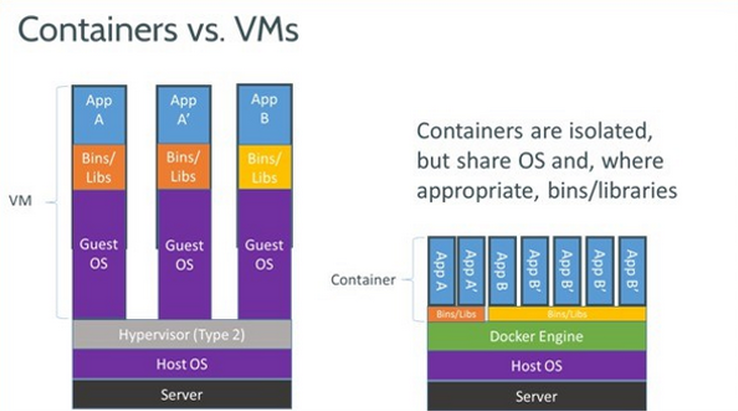
\includegraphics[scale=1.5]{images/vms-vs-containers.png} 
     	\vspace*{-0.5em}
		\caption{Differences between VMs and Docker containers}
	\end{figure}	
	
	\end{frame}	
	
	\section{Why using Docker?}
	
	
	\begin{frame}
	
	Thanks to Docker...
	\vspace*{0.6em}
	
	\begin{itemize}
		\item{There is \textbf{less dependency on systems} for testing applications 
			\begin{itemize}
				\item{No need to worry about your host OS installation, \textbf{containers have all the necessary to run in isolation everywhere}}				
			\end{itemize}					
		}	
		\item{Easy to \textbf{deploy applications with different versions} (one container: one version, another another version, etc.)}
		\item{\textbf{Robust to crashes} (if one application crashes th crash is contained in the container)}	
		\item{\textbf{Easy to productionalize applications} (an application based on Docker will work everywhere)}
		\item{\textbf{Easy to scale} (easy to add new containers to support a bigger charge)}
		\item{\textbf{Cheaper than VM} (lighter, takes less memory, faster, etc).}		
	\end{itemize}

	\end{frame}	
	
	\begin{frame}
	
	The \textbf{Docker Engine} is the program allowing us to create containers and install \textbf{ready-to-use environments} (Docker images). 
	\vspace*{0.6em}
	
	A little bit of vocabulary...
	\vspace*{0.6em}
	
    \begin{itemize}
	\item{The \textbf{host OS is the main operating system managing your machine} (Windows, MacOS, Linux)}  
	\item{The \textbf{Docker engine is the program that manages the containers}}   
	\item{A container is an \textbf{autonomous and isolated part of the host system, behaving as an independent machine}}
	\item{The \textbf{Docker client is the utility through which we transmit to the engine the commands to manage these containers}
		\begin{itemize}
			\item{It can be either from the command line (Docker CLI) or from a GUI (kitematic)}
		\end{itemize}			
	}   
    
    \end{itemize}  
	\end{frame}
	
	\begin{frame}	
	
	\begin{itemize}
		
	\item{A \textbf{Docker container needs very few resources because most system tasks are delegated to the host OS}}
	\item{Therefore: we can \textbf{multiply at low cost pseudo virtual machines} in which we could install "by hand" various software}
	\item{Fortunately, Docker offers pre-configured installations: \textbf{they are called images}
		\begin{itemize}
			\item{For example: images with pre-configured databases (Oracle, Postgresql, MySQL), Web servers (Apache, njnix), NoSQL servers (mongodb, cassandra), search engines (ElasticSearch, Solr), etc.}
		\end{itemize}			
	
	}
	\item{When instantiating a container: \textbf{an image is placed in a container} (the same image can be placed in several containers and thus obtain a distributed system)\footnotemark}
	
	
	\end{itemize}		

	\footnotetext{Which is very convenient for Data Engineering!}

	
	\end{frame}
	
	
	\section{How Docker works?}
	
	\begin{frame}
	
	\begin{figure}
		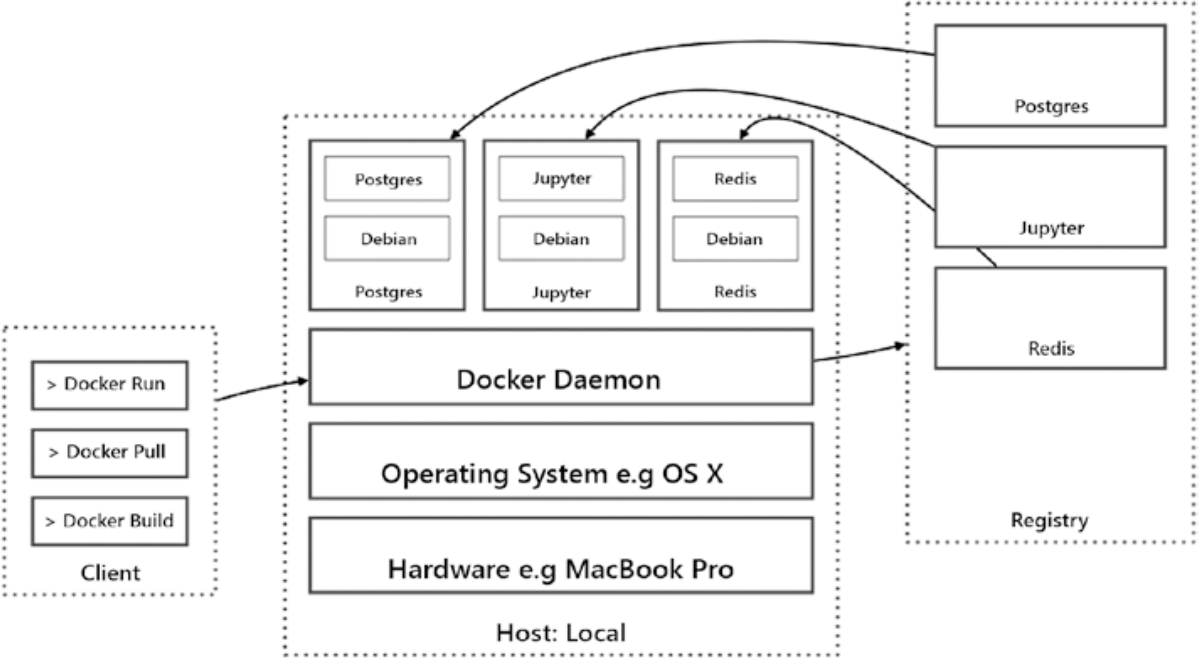
\includegraphics[scale=1.0]{images/docker-diagram.png} 
     	\vspace*{-0.5em}
		\caption{The docker ecosystem}
	\end{figure}		
	
	\footnotetext{The Docker Engine is often called Docker Daemon and vice-versa}	
	
	\end{frame}	
	
	\begin{frame}
	
	In order to understand how Docker works we have to briefly present the Docker ecosystem and how everything is related:
	\vspace*{0.6em}

%	You begin looking at Docker by focusing on the ecosystem of the container. Later, you will
%	leverage Docker’s tools for composing larger systems with the containers you have built.
%	In the immediate ecosystem of the Docker container, it is important to keep track of the following concepts:

	\begin{itemize}
	\item{The Docker client (mostly a CLI)}
	\item{The Host}
	\item{The Docker Engine (or Docker Daemon)}
	\item{Docker images}
	\item{Docker containers}
	\item{The Docker Registry}
	\item{Docker Compose (not in the diagram, will be explained later)}	
	\end{itemize}

	
	\end{frame}
	
	\begin{frame}
	\begin{itemize}	
	\item{The \textbf{Docker Client}: Mostly a command line interface used to \textbf{give instructions to the Docker engine} regardless of the details of the engine's implementation on your system (like a client-server architecture). The Docker client talks to the Docker engine that performs the work of containers and containerization (We will be using the Docker Client CLI)}
	\end{itemize}
	\begin{itemize}
	\item{The \textbf{Host}: The \textbf{host is a machine on which you will run the Docker Daemon/Engine}. Locally, the host will depend upon your Docker configuration. If you are running Docker for Linux, Docker for Mac, or Docker for Windows, the host will be your system itself}
\end{itemize}		
	
	\end{frame}	
	
	\begin{frame}
	
	\begin{itemize}
		\item{The \textbf{Docker Engine}: The Docker Engine is a persistent process managing all containers. It is running in a background service or daemon on the host. In fact, \textbf{the engine is occasionally referred to as the Docker Daemon}. The Docker Engine does the core work of Docker: \textbf{building, running, and distributing your Docker containers}. In this text, you will interact with the engine directly but will do so through the Docker Client}
		\item{The \textbf{Docker images and Docker containers}: The Docker Engine has several methods for building our own images. These include the Docker client and via a domain-specific language (DSL) known as the Dockerfile. We can also download images that other people have created. Docker containers are instances of Docker images.}	
	\end{itemize}		
		
	
	\end{frame}	
	
	\begin{frame}
	
	
	\begin{itemize}
		\item{The \textbf{Docker Registry}: Docker registries hold images. These are public or private stores from which you upload
or download images. For the purposes of this course, you will use the public Docker registry at Docker Hub. Docker Hub is the source of the official images of the major open source technologies you will be using including Jupyter, PostgreSQL, Redis, and MongoDB}
		\item{The \textbf{Docker Compose}: Docker Compose is a \textbf{tool for assembling applications consisting of multiple containers}. These applications are designed using a single YAML file and can be built, run, and scaled, each via a single command. Docker Compose is particularly useful for the data scientist in building standalone computational systems comprised of Jupyter and one or more databases}		
	\end{itemize}		
	
	\end{frame}		

	\section{Let's see how to use Docker}
	
	\begin{frame}[fragile]
	
	How to use the Docker Client to run containers?
	\vspace*{0.6em}
	
	In order to communicate with the Docker Engine, we can use a command line client program named simply docker. The simplest image is a "Hello World" image, we instantiate it with the following command:
	\begin{verbatim}
	$ docker run hello-world
	\end{verbatim}		
	
	The run is the command to instantiate a new image in a Docker container. Here is what you should get on the first run:
	
	\begin{verbatim}
	$ docker run hello-world

	Unable to find image 'hello-world:latest' locally
	latest: Pulling from library/hello-world
	4276590986f6: Pull complete
	Status: Downloaded newer image for hello-world:lates

	Hello from Docker!
	\end{verbatim}
		
	
	\end{frame}
	\begin{frame}[fragile]
		
	The list of the available images on your system can be obtained using the following command:
	\vspace*{0.6em}	
	
	\begin{verbatim}
	$ docker images
	\end{verbatim}
	
	Here is the type of output you should get now:
	\begingroup
    \fontsize{6pt}{12pt}\selectfont
	\begin{verbatim}
	REPOSITORY               TAG                 IMAGE ID            CREATED             SIZE
	hello-world              latest              4276590986f6        8 months ago        13.3kB	
	\end{verbatim}
	\endgroup

	You can instantiate an image and give it a name using the following command:
	\vspace*{0.6em}
	
	\begin{verbatim}
	$ docker run --name 'name-container' <options>	
	\end{verbatim}
		
	\end{frame}
	
	\begin{frame}[fragile]	
	
	Let's try now to run a basic container with a minimalist Ubuntu system:
	\vspace*{0.6em}
	
	\begin{verbatim}
	$ docker run -it ubuntu /bin/bash
	\end{verbatim}
	
	
	For more information about Docker-run:
	\vspace*{0.6em}	
	
	\begin{verbatim}
	$ man docker-run
	\end{verbatim}			
	
	The list of containers and their status can be obtained using:
	\vspace*{0.6em}
	
	\begin{verbatim}
	$ docker ps -a
	\end{verbatim}
	
	Example of output you could get:
	\vspace*{0.6em}
	
	\begingroup
    \fontsize{6pt}{12pt}\selectfont
	\begin{verbatim}
CONTAINER ID  IMAGE         COMMAND       CREATED         STATUS                      PORTS  NAMES
d1c2291dc9f9  mysql:latest  "docker..."   16 minutes ago  Exited (1) 9 minutes ago    3306   db
ec5215871db3  hello-world   "/hello"      19 minutes ago  Exited (0) 19 minutes ago          my test	
	\end{verbatim}
	\endgroup
		
	\end{frame}
	\begin{frame}[fragile]
	The first field "CONTAINER ID" tells us the identifier by which we can pass instructions to the container. 
	\vspace*{0.6em}
	
	Here are the most useful ones, assuming the container is d1c2291dc9f9. First of all we can stop it with the stop command:
	\vspace*{0.6em}
	
	\begin{verbatim}
	$ docker stop d1c2291dc9f9
	\end{verbatim}
	
	Stopping a container does not mean that it no longer exists, but that it is no longer active. You can restart it with the start command:
	\vspace*{0.6em}	
	
	\begin{verbatim}
	$ docker start id_container
	\end{verbatim}		

	To remove it, it is the docker rm command. \
	To inspect the system/network configuration of a container, Docker provides the inspect command:
	\vspace*{0.6em}
	
	\begin{verbatim}
	$ docker inspect id_container
	\end{verbatim}
	
	We obtain a large JSON document. Among all the information given, the IP address of the container is particularly interesting. We get it with:
	\vspace*{0.6em}
	
	\begin{verbatim}
	$ docker inspect <id_container> | grep "IPAddress"
	\end{verbatim}
	
		
	\end{frame}
	\begin{frame}[fragile]

	\textbf{Docker provides a publishing mechanism to indicate on which port a container is listening}. 
	You simply indicate with the --publish (or -p) option how to associate a container port with a host system port. 
	--detach (or -d) indicates that the container is launched in the background, which avoids blocking the terminal	
	\vspace*{0.6em}
	
	In case your container contains a server (a http server):
	\vspace*{0.6em}	
	
	\begin{verbatim}	
	$ docker run --name web2 --publish 81:80 --detach httpd:latest
	\end{verbatim}
	
	Or simply:
	\vspace*{0.6em}
	
	\begin{verbatim}
	$ docker run --name web2 -p 81:80  -d httpd
	\end{verbatim}		
	
	The -p option indicates that port 80 of the container is forwarded to port 81 of the host machine.
	
	\end{frame}
	\section{Let's make your own Docker image}
	\begin{frame}
	
	\begin{itemize}
	\item{Every Docker Image is \textbf{defined as a stack of layers} each defining \textbf{fundamental, stateless changes} to the image:
		\begin{itemize}
			\item{The \textbf{first layer might be a minimalist operating system image} (Debian, Ubuntu, etc. Docker image)}
			\item{The \textbf{next layer is the installation of dependencies necessary for your application to run} and all the way up to the source code of your application}
		\end{itemize}			
	}
	\item{The file named "\textbf{Dockerfile}" permits to \textbf{define the layers of the image and thus build the image}:
		\begin{itemize}
			\item{The file uses a domain-specific language to tell the Docker daemon how to sequentially build a Docker image}
			\item{All the instructions contained in Dockerfile are read and executed one by one to build the image}
		\end{itemize}
	
	}
	\end{itemize}	
	
	
	\end{frame}	
	
	\subsection{Best practices}
	\begin{frame}
	
	When writing a Dockerfile one should follows the following best practices:
	\vspace*{0.6em}
	
	\begin{itemize}
	\item{\textbf{Containers should be ephemeral or stateless} in that they can be re-instantiated with a minimum of set up and configuration}
	\item{\textbf{Avoid installing unnecessary packages}}
	\item{Each container \textbf{should have only one purpose} (ex: a database, a web server, etc.)}
	\item{The \textbf{number of layers should be minimized}}
	\end{itemize}	

	\end{frame}


	\begin{frame}

	About statelessness:
	\vspace*{0.6em}

	\begin{itemize}
	\item{An \textbf{application may run more than one container at a time}
		\begin{itemize}
			\item{All these containers \textbf{should be stateless}}
		\end{itemize}			
	}
	\item{If info is to be persisted beyond the termination of the container it \textbf{should be written to a stateful backing service such as a database} (like MongoDB or Postgres) or a key-value store (like Redis)}
	\item{Indeed: We \textbf{should be able to shut down a container and remove it from our system}, then \textbf{start an identical container using the same image}, and \textbf{run command with no effect to our work}}
\end{itemize}		 

	\end{frame}
	\subsection{How to create a Dockerfile?}
	\begin{frame}[fragile]
	The first thing you have to do is to \textbf{create a file named "Dockerfile"} then define in it the image you are going to use as a base, thanks to the \textbf{FROM} statement. In our case, we will use a \textbf{Ubuntu base image}\footnote{To find the list of the docker images you can use as base images you can go here: $https://hub.docker.com/$}.
	
	\begin{verbatim}
	FROM ubuntu
	\end{verbatim}
	
	The \textbf{FROM} statement can only be used once in a Dockerfile!
	
	You can add the name and coordinate of the maintainer of the Dockerfile with:
	\begin{verbatim}
	MAINTAINER Firstname Lastname (mail@mymail.com)	
	\end{verbatim}

	\end{frame}
	\begin{frame}[fragile]
	Then you can use the \textbf{RUN} instruction to execute command lines in your container, for example updating the Ubuntu system and installing mongodb:
	
	\begin{verbatim}
	RUN apt-get update 
	RUN apt-get install mongodb 
	\end{verbatim}

	\begin{block}{Notes}
	\textit{apt-get} is a Ubuntu/Debian package manager, you can use it to search, install, update or remove software. The package manager your can use depend on the base image you use (for instance, of your base image is archlinux, you have to use pacman)
	\end{block}

	The \textbf{ENV} instruction permits to set or update environment variables (like PATH, etc).	
	
	\end{frame}
	\begin{frame}[fragile]
	
	Then use the \textbf{ADD} statement to copy or upload files to the image. In our case, we use it to add the sources of our local application in the /app/ folder of the image.
	\vspace*{0.6em}	
	
	\begin{verbatim}
	ADD . /PATH_IN_CONTAINER/
	\end{verbatim}
	
	Then use the \textbf{WORKDIR} command to change the current directory. The command is equivalent to a cd command on the command line. All the commands that follow will be executed from the defined directory.
	\begin{verbatim}
	WORKDIR /PATH_IN_CONTAINER	
	\end{verbatim}		
	
	\end{frame}
	\begin{frame}[fragile]
	Now that the source code and dependencies are present in your container, we need to tell our image some final information.
	
	\begin{verbatim}
	EXHIBIT 27017
	VOLUME /PATH_IN_CONTAINER_TO_SOME_REPOSITORY
	\end{verbatim}
	
	The \textbf{EXPOSE} statement is used to indicate the port on which your application is listening. The \textbf{VOLUME} statement is used to indicate which directory you want to share with your host.	
	\vspace*{0.6em}
	
	We will conclude with the instruction that must always be present, and place it in the last line for better understanding: \textbf{CMD}. It allows our container to know which command it should execute when it starts.
	
	\begin{verbatim}
	CMD sudo systemctl start mongodb	
	\end{verbatim}
	
	\end{frame}
		
	\begin{frame}[fragile]
	
	Put everything together, the Dockerfile file looks like:
	\vspace*{0.6em}
	
	\begin{verbatim}
	FROM ubuntu
	MAINTAINER Firstname Lastname (mail@mymail.com)
	RUN apt-get update
	RUN apt-get install mongodb
	ADD . /app/ 
	WORKDIR /app
	EXPOSE 27017
	VOLUME /app/logs
	CMD  sudo systemctl start mongodb	
	\end{verbatim}				
	
	\end{frame}
	\begin{frame}[fragile]
	You can now create your first own Docker image!
	\vspace*{0.6em}
	
	Type this command in the repository containing the Dockerfile file:
	\begin{verbatim}
	$ docker build -t my-mongodb-image .
	\end{verbatim}
	
	The -t argument allows you to give a name to your Docker image. This makes it easier to find your image later.
	The . is the directory where the Dockerfile is located. In our case, at the root of our project. 
	\vspace*{0.6em}

	Now you can launch your container with the docker run command like this:

	\begin{verbatim}
	$ docker run -d -p 27017:27017 my-mongodb-image
	\end{verbatim}
	
	
	\end{frame}
	\section{Create application with Docker Compose}
	\begin{frame}[fragile]
		
	A full application requires the assembly of several containers.
	\vspace*{0.6em} 
	
	For example: for a dynamic website you may need a database (MySQL), a web-server (Apache) and a scripting language interpreter (PHP). In that case you need three containers: the \textbf{application is then the assembly of these three containers} together.
	\vspace*{0.6em}
	
	With Docker compose we can create a multi-container architecture that we can call "stack". This Stack will be :
	\vspace*{0.6em}
	
	\begin{itemize}
	\item{Autonomous (because it is ready to be "set up" everywhere, whatever the target platform)}
	\item{Pre-parameterized (everything is in the docker-compose.yml file)}
	\item{Isolated (all services are not necessarily publicly accessible, but are accessible by your other applications)}
	\item{Easily manageable with the CLI (docker-compose up/down/start/stop)}
	\end{itemize}
	
	\end{frame}
	
	\begin{frame}
	
	In order to define a multi-container Docker application we have to write a docker-compose.yml file. ".yml" is the extension of a text file formatted in YAML (formatted explicited below) :
	\vspace*{0.6em}
	
	The syntax of the YAML stream is relatively simple and efficient. It has been established to be as readable as possible by humans:
	\vspace*{0.6em}
	
	\begin{itemize}
	\item{Comments are indicated by the hash sign (\#) and extend over the whole line}
	\item{List elements are denoted by a dash (-) followed by a space, with one element per line.}
	\item{Arrays are of the form "key : value", with one pair per line.}
	\item{Scalars can be surrounded by double quotes (") or single quotes (')}
	\item{etc.}		
	\end{itemize}
			
	
	\end{frame}
	\begin{frame}[fragile]
	
	First thing to do when writing a docker-compose.yml file is to \textbf{write the version of Docker Compose} you use:
	\vspace*{0.6em}
	
	\begin{verbatim}
	version: '3'
	\end{verbatim}
	
	This instructs Docker Compose that we're using version 3 of the tool. The next line will instruct Docker Compose that what follows will be \textbf{the services to deploy}. That is defined with: 
	
	\begin{verbatim}
	services:
	\end{verbatim}
	\end{frame}
	\begin{frame}[fragile]
	
	Let's imagine we want to build an application with a web server and a MongoDB database.
    Our first section to define will be the web portion of the stack. We can do this with two simple lines: 
    
    \begin{verbatim}
	web:
	    image: http 
    \end{verbatim}    
    
	What the above does is instruct Docker Compose to deploy a container using the official http Docker image. We're not doing anything special for this container. It's just basic. 
	\vspace*{0.6em}
       
Our next section will define a database. This one gets a bit more complicated, as we must configure the necessary parameters for the database to function. We begin by defining the section with:
\vspace*{0.6em}

	\begin{verbatim}
	db:
	     image:mongodb
	\end{verbatim}
		
	\end{frame}
	\begin{frame}[fragile]	
	
	Now we define both the external and internal ports to use for the database. For this we'll make use of the default MongoDB ports and define them: 
	\vspace*{0.6em}
	
	\begin{verbatim}
	ports:
	     - "27017-27019:27017-27019"
	\end{verbatim}
	
Why do we write the port two time?
The \textbf{first port is the port on the host machine} and the \textbf{second the port in the container} (we can map the default port of the server to different ports of the host machine and thus have several mongodb servers in multiple containers).
\vspace*{0.6em}

Finally, we configure the database environment. The environment will be the configuration options for the database (passwords, users, database name):
\vspace*{0.6em}

	\begin{verbatim}
	environment:
 	   -MONGO_INITDB_DATABASE=mongo_db_name
 	   -MONGO_INITDB_ROOT_USERNAME=mongo_db_username  
 	   -MONGO_INITDB_ROOT_PASSWORD=mongo_db_password
	\end{verbatim}
	
	
	\end{frame}
	\begin{frame}[fragile]
	Putting everything together gives:
	\vspace*{0.6em}
	
	\begin{verbatim}
version: '3'
services:
  web:
    image: http
    container_name :"WEB Server"
    ports :
    - "80:80"
  db:
    image: mongo
    container_name :"Mongo DB"
    ports:
      - "27017-27019:27017-27019"
    environment:
   	  - MONGO_INITDB_DATABASE=mongo_db_name
      - MONGO_INITDB_ROOT_USERNAME=mongo_db_username
      - MONGO_INITDB_ROOT_PASSWORD=mongo_db_password
	\end{verbatim}
	
	\end{frame}
	\begin{frame}[fragile]
	Now that you have created your docker-compose.yml file you can run the application by typing:
	\vspace*{0.6em}

	\begin{verbatim}
	$ docker-compose up 
	\end{verbatim} 

	This must be typed inside the repository containing the docker-compose.yml\footnote{The complete and offical documentation about Docker Compose: https://docs.docker.com/compose/} file.
	You can also run your application in detached mode using -d:
	\vspace*{0.6em}

	\begin{verbatim}
	$ docker-compose up -d
	\end{verbatim}
	
	Later you can stop it using:
	\vspace*{0.6em}
	
	\begin{verbatim}
	$ docker-compose stop
	\end{verbatim}
	
	You can bring everything down, removing the containers entirely, with the down command:
	\vspace*{0.6em}
	
	\begin{verbatim}
	$ docker-compose down
	\end{verbatim}

	

	\end{frame}
	\begin{frame}
	
	That's all for today!
	\vspace*{0.6em}
	
	Please install the following software on your own system for the next session (not your VM!):
	\begin{itemize}
	\item{Docker}
	\item{Docker Compose}
	\item{For Windows users: git bash (https://gitforwindows.org/)}
	\item{You may also install: Kitematic (optional: we will not use it)}
	\end{itemize}		
		
	
	
	
			
	
		
	
	\end{frame}
	\end{document}	
	